% pdfLaTeX is the engine selected by the supplied Overleaf template.
% This narrow compatibility block also lets the bundled XeTeX preview engine
% render the same class. It maps the template's spot blue to its CMYK value.
% The IEEE class files themselves stay unchanged.
\ifdefined\XeTeXversion
  \RequirePackage[T1]{fontenc}
  \RequirePackage{color}
  \makeatletter
  \@namedef{ver@spotcolor.sty}{2026/10/11 XeTeX compatibility}
  \newcommand{\NewSpotColorSpace}[1]{}
  \newcommand{\AddSpotColor}[4]{}
  \newcommand{\SetPageColorSpace}[1]{}
  \def\SpotSpace{ }
  \def\color@spotcolor#1#2{\color@cmyk#1{1,.3,0,.2}}
  \makeatother
\fi
% IEEE Access defines a metadata command named \year. PGF needs the TeX
% primitive while its packages initialize, so preserve it temporarily.
\let\primitiveyear\year
\documentclass[nolineno]{ieeeaccess}
\let\accessyear\year
\let\year\primitiveyear
\usepackage[utf8]{inputenc}
\usepackage{cite}
\usepackage{amsmath,amssymb,amsfonts}
\usepackage{graphicx}
\usepackage{textcomp}
\usepackage{booktabs}
\usepackage{etoolbox}
\usepackage{tikz}
\usetikzlibrary{arrows.meta,positioning}
\let\year\accessyear
\ifdefined\XeTeXversion
  \definecolor{accessblue}{cmyk}{1,.3,0,.2}
\fi
% The class's caption formatter normally receives this width from \Figure.
% The code-native figure has one-column width.
\def\xfigwd{\columnwidth}

% Keep the IEEE Access layout. Replace journal publication metadata with course metadata.
\makeatletter
\patchcmd{\@maketitle}{{\vss\doifont Digital Object Identifier\space\@doi\vss}\vspace*{7.4mm}\par}{}{}{\errmessage{Could not remove journal DOI metadata}}
\def\proposalfooter{\hbox to \textwidth{\footervolfont Project 2 Research Proposal\hfill\footerpagefont\thepage}}
\def\ps@titlepage{\def\@oddhead{\hfill\headerlogo}\let\@evenhead\@oddhead
  \def\@oddfoot{\proposalfooter}\let\@evenfoot\@oddfoot}
\def\ps@headings{\def\@oddhead{\hbox to \textwidth{\headerfont Differential Privacy in Federated Learning: An Accuracy and Runtime Benchmark\hfill}}
  \let\@evenhead\@oddhead\def\@oddfoot{\proposalfooter}\let\@evenfoot\@oddfoot}
\makeatother
\pagestyle{headings}

\begin{document}
\history{Research area: Privacy-Preserving Cryptography. Approach: Experimental Analysis. Submission: October 12, 2026.}
\doi{}
\title{Differential Privacy in Federated Learning: An Accuracy and Runtime Benchmark}
\author{\uppercase{Mateo O\~nate} and \uppercase{Demian Viteri}}
\address{Yachay Tech University, School of Mathematical and Computational Sciences, Ecuador}
\tfootnote{Cryptography. Prof. Cristhian Iza.}
\markboth{Differential Privacy in Federated Learning: An Accuracy and Runtime Benchmark}{Differential Privacy in Federated Learning: An Accuracy and Runtime Benchmark}
\corresp{}

\begin{abstract}
Federated learning keeps training records at participating clients, but the model updates they share can still expose information about those records. Differential privacy limits this exposure through controlled randomness, at a cost to model accuracy and training time. This project proposes a small experimental benchmark to measure this trade-off for handwritten digit classification. Ten clients will train a softmax model in a single-computer simulation. The benchmark will compare ordinary federated averaging, a clipping-only control, and three settings of differentially private stochastic gradient descent. The experiments will cover both randomly distributed data and data concentrated by digit label. Each private setting will have a fixed privacy target, and an accountant will track its cumulative cost across all training rounds. Three repetitions of every configuration will provide accuracy, privacy bounds, runtime, and memory measurements. The goal is to identify the lowest tested privacy budget with an acceptable accuracy loss, or document when none meets the predefined criterion. The project will produce a reproducible benchmark and a practical account of its limits, without requiring specialized hardware or sensitive personal data.
\end{abstract}

\begin{keywords}
Benchmarking, differential privacy, federated learning, privacy-preserving machine learning.
\end{keywords}
\titlepgskip=-15pt
\maketitle

\section{Problem and Motivation}
Federated averaging (FedAvg) trains a shared model through local updates, while each client retains its training records~\cite{mcmahan}. This separation is useful, but it does not establish a privacy guarantee. Prior research reconstructed training examples from shared gradients under specific attack conditions~\cite{zhu}. This result motivates protection for the information leaving a client, even when no raw image travels to the server.

Differential privacy (DP) bounds the change in an algorithm's output distribution when one protected record changes~\cite{dwork}. Established private training procedures combine per-example gradient clipping, Gaussian noise, and privacy accounting~\cite{abadi}. Related research has also examined record-level DP in federated training~\cite{zheng}. However, the privacy budget alone does not indicate the accuracy loss of a particular model or the additional computation it requires.

The project will measure those costs under a small, controlled setup suitable for reproduction on a personal computer. The analysis will examine data heterogeneity and separate the effect of clipping from the effect of noise. The study evaluates established methods and does not propose a new privacy mechanism. This scope allows time for accountant verification, repeated experiments, and interpretation of the results.

\section{Research Question and Objectives}
\textbf{Research question:} For a fixed softmax classifier and training schedule, how do record-level DP budgets affect test accuracy and runtime in FedAvg, and how does label-skewed client data change this trade-off?

The project has three objectives:
\begin{enumerate}
  \item Implement a reproducible FedAvg simulation with ordinary, clipping-only, and private local training.
  \item Measure accuracy, cumulative privacy bounds, runtime, and memory under two client data distributions and three private budgets.
  \item Identify a practical setting under a predefined accuracy-loss criterion, and document the conditions where it fails.
\end{enumerate}

\newpage
\section{Proposed Methodology}
\subsection{Dataset and Computing Setup}
The benchmark will run in Python with PyTorch, torchvision, and Opacus, whose implementation supports per-example gradients and private training~\cite{opacus}. A single computer will execute ten simulated clients sequentially. The experimental records will include its processor, memory, operating system, library versions, and CPU thread count. The simulation will exchange model parameters in memory. Its timing will measure computation, not physical network latency.

The dataset will consist of MNIST handwritten digits~\cite{lecun}. Sampling from its training split will provide 10,000 images, balanced across the ten labels, and a separate 2,000-image public validation set. The official 10,000-image test split will remain separate. Each client will hold 1,000 training images. The IID condition will distribute images randomly. The non-IID condition will sort images by label, form twenty 500-image shards, and assign two shards to each client, following the label-skewed benchmark idea in~\cite{mcmahan}. Both allocations will remain fixed throughout each run.

\subsection{Model and Local Training}
The classifier will map 784 normalized pixel values to ten logits through one linear layer with 7,850 trainable parameters. This model keeps CPU experiments manageable and makes the training procedure easy to inspect. Every client will participate in each of ten rounds. Clients will start from the same global weights, train locally, and return their weights for equal-weight averaging.

Each round will contain sixteen local optimizer steps. The configuration will request a nominal batch size of 64 and apply Poisson sampling in all five settings. For 1,000 records, the planned sampling rate is $q=1/16$, with an expected batch size of 62.5. Verification will cover the actual rate reported by the loader. The initial optimizer will be SGD with learning rate 0.1 and no momentum. A pilot on the separate public validation set will check convergence and runtime. Any revised shared training settings will remain fixed during the full comparison, without selection based on test results.

\begin{figure}[t]
\centering
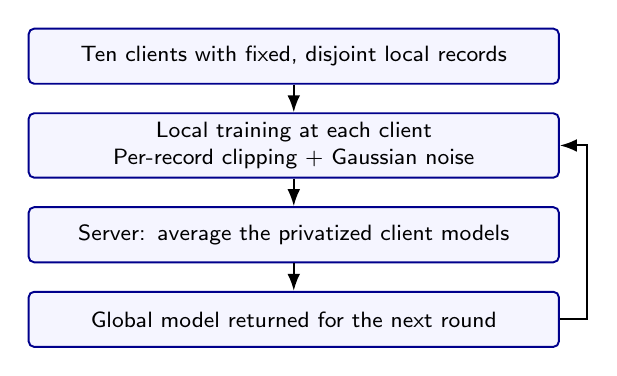
\begin{tikzpicture}[font=\sffamily\footnotesize,>=Latex,
  box/.style={draw=blue!55!black,fill=blue!4,rounded corners=2pt,align=center,text width=6.5cm,minimum height=0.7cm},
  every path/.style={line width=0.7pt}]
\node[box] (data) {Ten clients with fixed, disjoint local records};
\node[box,below=0.35cm of data] (train) {Local training at each client\\Per-record clipping + Gaussian noise};
\node[box,below=0.35cm of train] (server) {Server: average the privatized client models};
\node[box,below=0.35cm of server] (model) {Global model returned for the next round};
\draw[->] (data) -- (train);
\draw[->] (train) -- (server);
\draw[->] (server) -- (model);
\draw[->] (model.east) -- ++(0.35,0) |- (train.east);
\end{tikzpicture}
\caption{Planned private-training path. Noise enters before a model leaves its client. An accountant at each client persists across rounds.}
\label{fig:pipeline}
\end{figure}

\subsection{Privacy Mechanism and Threat Model}
The threat model considers an honest-but-curious server. It follows the protocol but can inspect every client model it receives. Clients apply record-level DP-SGD before releasing those models, as shown in Fig.~\ref{fig:pipeline}. The protected unit is one image, not an entire client or every image from one writer. Neighboring datasets differ by adding or removing one record within a fixed client allocation. Public sampling settings and aggregation weights stay fixed. The privacy claim excludes the label-based partition construction itself.

For each sampled image, DP-SGD computes a gradient and limits its $L_2$ norm to $C=1$. It adds Gaussian noise with standard deviation $\sigma C$ to the sum of clipped gradients, then divides by a fixed public normalization factor~\cite{abadi}. The experiment log will record the optimizer's actual factor, which need not equal the expected Poisson batch size exactly. Opacus will calibrate $\sigma$ with its R\'enyi DP accountant for all 160 steps, targeting $\epsilon\in\{2,4,8\}$ at $\delta=10^{-5}$. At fixed $\delta$, smaller $\epsilon$ gives a tighter bound on how much one record can affect observable outputs~\cite{dwork}. These numbers are bounds, not percentages of information hidden.

Each client will retain one R\'enyi DP accountant through all 160 local steps, including when global weights replace local weights~\cite{mironov}. The analysis will report the achieved per-client bounds and their maximum for the complete sequence of client models observed and global models released in one run. With fixed, disjoint client records, a neighboring change affects one client's private accesses. The other computations are conditional post-processing, so the maximum gives the bound for that run~\cite{dwork}. Full participation gives no amplification from client selection.

The budgets refer to separate runs. Publishing multiple models trained on the same private records would require additional composition. Because MNIST is public and the controls are non-private, the study does not claim a DP guarantee for the entire benchmark release. Secure aggregation, protection of a compromised client, and active attacks fall outside this study.

\subsection{Experimental Matrix and Correctness Checks}
Table~\ref{tab:design} defines five training settings. The clipping-only control will help attribute accuracy loss to clipping or added noise. Two distributions and three independent repetitions produce $5\times2\times3=30$ complete runs. Within each repetition, settings will share the data allocation, starting model, sampling policy, and step count. DP sampling and noise will have independent randomness.

\begin{table}[t]
\caption{Planned training settings. Every row runs under IID and label-skewed allocations with three repetitions.}
\label{tab:design}
\centering
\small
\setlength{\tabcolsep}{4pt}
\begin{tabular}{lccc}
\toprule
\textbf{Setting} & \textbf{Clipping} & \textbf{Noise} & \textbf{Target $\epsilon$}\\
\midrule
Ordinary FedAvg & No & None & No DP bound\\
Clipping-only & $C=1$ & None & No DP bound\\
DP-SGD, tighter & $C=1$ & Calibrated & 2\\
DP-SGD, middle & $C=1$ & Calibrated & 4\\
DP-SGD, looser & $C=1$ & Calibrated & 8\\
\bottomrule
\end{tabular}
\end{table}

Before the full experiment, correctness checks will confirm that client partitions and evaluation splits do not overlap, compare the model average against a small hand-computed example, and verify per-record clipping on synthetic gradients. Additional checks will cover the loader's sampling rate, cumulative accountant step count, and final budget after repeated global-weight reloads. The experiment configuration will include a record of these checks.

\section{Evaluation Plan and Expected Outcomes}
The evaluation will assess the final model after the fixed tenth round. The main utility metric will be test accuracy, reported as the mean and sample standard deviation of three runs, alongside individual observations. Accuracy loss will be the difference in percentage points from clipping-only FedAvg under the same allocation and repetition. Comparing clipping-only with ordinary FedAvg will quantify the clipping effect.

Privacy reporting will include achieved $\epsilon$, fixed $\delta$, noise multiplier, sampling rate, and total steps. Resource measurements will cover training wall-clock time in seconds and peak resident memory in MiB in a fresh process for each run. Timing will exclude dataset downloading and final testing, but include local updates, aggregation, and privacy operations. Configuration order will alternate, while the CPU thread count will remain fixed. Runtime overhead will be the private-to-ordinary training-time ratio on the same computer.

The principal plots will show accuracy against achieved privacy budget, accuracy by round on the public validation set, and runtime overhead. Tighter budgets are expected to require more noise and usually reduce accuracy. Label skew is also expected to affect training, but the size and direction of its interaction with DP are empirical questions. The proposal does not assume a numerical performance result in advance.

For each allocation, the analysis will identify the lowest tested budget whose mean paired accuracy loss is at most five percentage points from the clipping-only control. Reporting will include the variability of that loss and explicitly state when no setting meets the criterion. Three repetitions support a descriptive comparison, not broad claims of statistical significance. Findings will apply to this model, dataset, schedule, and computer.

\section{Work Plan and Deliverables}
The work plan spans four working weeks within the term. Week 1 will cover the literature review, data splits, and FedAvg pilot. Week 2 will focus on private training integration and accountant verification. Week 3 will cover the 30 runs and any documented reruns needed for execution failures. Week 4 will cover plot preparation, interpretation of the comparisons, and report writing. Cross-review of implementation checks and analytical conclusions will support the final report.

The deliverables will include runnable scripts, fixed configuration files, public partition and initialization seeds, per-run metric files, and the final report. A pilot will determine the actual computing budget. If runtime is excessive, the revised protocol will reduce the common number of rounds before the full experiment, recalibrate every private setting, and document the change. Both data conditions, all five settings, and three repetitions will remain in the design. The report will distinguish public benchmark reproducibility from a private deployment, where disclosing noise or sampling randomness can invalidate protection.

\begin{thebibliography}{8}
\bibitem{mcmahan}
H. B. McMahan, E. Moore, D. Ramage, S. Hampson, and B. Ag\"uera y Arcas, ``Communication-efficient learning of deep networks from decentralized data,'' in \emph{Proc. AISTATS}, PMLR, vol. 54, 2017, pp. 1273--1282.
\bibitem{zhu}
L. Zhu, Z. Liu, and S. Han, ``Deep leakage from gradients,'' in \emph{Advances in Neural Information Processing Systems}, vol. 32, 2019.
\bibitem{dwork}
C. Dwork and A. Roth, ``The algorithmic foundations of differential privacy,'' \emph{Foundations and Trends in Theoretical Computer Science}, vol. 9, nos. 3--4, pp. 211--407, 2014, doi: 10.1561/0400000042.
\bibitem{abadi}
M. Abadi et al., ``Deep learning with differential privacy,'' in \emph{Proc. ACM CCS}, 2016, pp. 308--318, doi: 10.1145/2976749.2978318.
\bibitem{zheng}
Q. Zheng, S. Chen, Q. Long, and W. J. Su, ``Federated $f$-differential privacy,'' in \emph{Proc. AISTATS}, PMLR, vol. 130, 2021, pp. 2251--2259.
\bibitem{opacus}
A. Yousefpour et al., ``Opacus: User-friendly differential privacy library in PyTorch,'' \emph{arXiv preprint arXiv:2109.12298}, 2021.
\bibitem{lecun}
Y. LeCun, L. Bottou, Y. Bengio, and P. Haffner, ``Gradient-based learning applied to document recognition,'' \emph{Proceedings of the IEEE}, vol. 86, no. 11, pp. 2278--2324, 1998, doi: 10.1109/5.726791.
\bibitem{mironov}
I. Mironov, ``R\'enyi differential privacy,'' in \emph{Proc. IEEE CSF}, 2017, pp. 263--275, doi: 10.1109/CSF.2017.11.
\end{thebibliography}
\EOD
\end{document}
